\documentclass[11pt]{article}

\usepackage[utf8]{inputenc}
\usepackage[T1]{fontenc}
\usepackage[protrusion=true,expansion=false]{microtype}
\usepackage{amsmath,amssymb,amsthm}
\usepackage{mathtools}
\usepackage{stmaryrd}
\usepackage{enumitem}
\usepackage{booktabs}
\usepackage{array}
\usepackage{longtable}
\usepackage{xcolor}
\usepackage{listings}
\usepackage[margin=1in]{geometry}
\usepackage[hidelinks]{hyperref}
\usepackage{tikz}
\usetikzlibrary{arrows.meta,positioning,calc,shapes.geometric}

% ---- theorem environments ----
\newtheorem{definition}{Definition}[section]
\newtheorem{remark}{Remark}[section]
\newtheorem{proposition}{Proposition}[section]
\newtheorem{invariant}{Invariant}[section]

% ---- notation ----
\newcommand{\proc}[1]{\mathsf{#1}}
\newcommand{\name}[1]{\mathtt{#1}}
\newcommand{\quoteP}[1]{\ulcorner #1 \urcorner}
\newcommand{\deref}[1]{{\ast}#1}
\newcommand{\bnf}{\mathrel{::=}}
\newcommand{\sigj}{s_{1}\!\ast\! s_{2}}
\newcommand{\R}{\mathbb{R}}
\newcommand{\N}{\mathbb{N}}
\newcommand{\Csig}{\mathsf{C}}
\newcommand{\Kcut}{\mathsf{K}}
\newcommand{\sep}{\mathbin{\ast}}
\newcommand{\colsep}{\;\big|\;}
\newcommand{\bigsep}{\mathop{\vphantom{\sum}\text{\Large$\ast$}}\displaylimits}
\DeclareMathOperator{\Demand}{\Delta}
\DeclareMathOperator{\Supply}{\Sigma}

% ---- listings setup for rholang-flavoured pseudocode ----
\definecolor{codekw}{rgb}{0.10,0.10,0.55}
\definecolor{codecomment}{rgb}{0.30,0.45,0.30}
\definecolor{codestr}{rgb}{0.55,0.20,0.10}
\lstdefinelanguage{rholang}{
  morekeywords={new,in,for,contract,match,if,else,true,false,Nil,select,let,bundle},
  sensitive=true,
  morecomment=[l]{//},
  morecomment=[s]{/*}{*/},
  morestring=[b]",
}
\lstset{
  language=rholang,
  basicstyle=\ttfamily\footnotesize,
  keywordstyle=\color{codekw}\bfseries,
  commentstyle=\color{codecomment}\itshape,
  stringstyle=\color{codestr},
  numbers=left,
  numberstyle=\tiny\color{gray},
  numbersep=7pt,
  showstringspaces=false,
  breaklines=true,
  frame=single,
  framerule=0.3pt,
  rulecolor=\color{gray!50},
  columns=fullflexible,
  keepspaces=true,
  xleftmargin=1.2em,
  aboveskip=0.8em,
  belowskip=0.8em,
}

\title{\textbf{Prediction Markets on the Cost-Accounted Rho Calculus}\\[0.3em]
\large A gap analysis, an oracle discipline, a market-launch configuration tuple,\\
and an implementation blueprint for a Kalshi/Polymarket-class venue on F1R3Fi}

\author{L.\,G.\ Meredith\\
F1R3FLY.io \quad \href{mailto:lgreg.meredith@f1r3fly.io}{lgreg.meredith@f1r3fly.io}}

\date{June 2026}

\begin{document}
\maketitle

\begin{abstract}
The Peyton Jones--Eber--Seward combinators, realised in the cost-accounted rho calculus,
give an executable, resource-safe settlement language for financial \emph{instruments}. A
prediction market, however, is a \emph{venue}, and a venue is mostly the three things the
combinator language deliberately does not model: a fungible bearer-position layer, a
matching/automated-market-maker microstructure, and a resolution oracle robust against an
adversarial, informally-specified world. This note closes that distance. We inventory the
gaps between the existing F1R3Fi realisation and a venue with feature parity to Kalshi and
Polymarket; we show that the position layer falls out of located purses and the acceptance
gate almost for free (the Gnosis conditional-token conservation law \emph{is} a linear
funding proof); we give an oracle discipline in which a trusted computation lives behind a
channel, non-repeatable oracle calls are secured not by replicated determinism---unattainable
for, e.g., a high-temperature language model---but by \emph{validator attribution}, a blame
capability that Casper-style accountable safety already supplies, with the oracle's
declared \emph{specification} furnishing the falsification surface that lets blame attach;
we present the market launch as a single \emph{dependent configuration tuple} whose policy
fields are freely chosen above a fixed floor of safety invariants the type discipline
discharges uniformly; we specify the maker microstructure as two orthogonal axes (pricing
rule $\times$ execution discipline) and develop the batch-cleared variant as the form
idiomatic to concurrent acceptance over disjoint token pools; and we give the
resolution-latch state machine in full, with redeem nested below both consensus finality
(the Casper finality fringe, which the runtime already computes for garbage collection) and
dispute finality (a window measured in finalised time). Throughout, every required component
is shown to map onto apparatus already present in cost-accounted rho plus the combinators;
the one genuinely new build is the maker, which is engineering on the substrate rather than
an extension of it. The note is written to be implementation-grade: a competent engineer or
agent should be able to build from it.
\end{abstract}

\tableofcontents
\bigskip

\section{Introduction}\label{sec:intro}

A financial contract, in the Peyton Jones--Eber--Seward sense~\cite{spj}, is a thing one
\emph{holds}: an agreement to exchange cash flows contingent on time and on observable
quantities, generated from a handful of combinators (\textsf{zero}, \textsf{one},
\textsf{give}, \textsf{and}, \textsf{or}, \textsf{scale}, \textsf{truncate}, \textsf{get}).
The companion note~\cite{finrho} realises those combinators in the cost-accounted rho
calculus~\cite{cost,cigslt}---the reflective higher-order process calculus that is the
formal core of Rholang~\cite{rholang}---and shows that the realisation turns a
description-and-valuation language into an executable settlement language whose executions
are resource-safe and atomic by construction. Located authority over funds, atomicity of
multi-step settlement, and a linear resource proof discharged before any step fires are the
three things the construction supplies that a denotational semantics cannot.

A prediction market is a different kind of object. It is not an instrument but a
\emph{venue}: a place where many anonymous participants trade fungible, bearer claims on the
outcome of a future event, against one another or against an automated maker, with the claims
redeemed for collateral once the event is recognised to have occurred. Kalshi and Polymarket
are the two reference points. Kalshi is a regulated, central-limit-order-book exchange whose
markets resolve against designated sources under a compliance regime; Polymarket is a
permissionless venue whose outcome tokens follow the Gnosis conditional-token pattern, whose
liquidity is provided by a constant-product maker and an off-chain order book, and whose
markets resolve through UMA's optimistic, bonded oracle. Between them they span the design
space we must cover.

The thesis of this note is that the F1R3Fi substrate is unusually well-suited to building
such a venue, that most of what a venue needs is \emph{already present} in the
cost-accounted calculus, and that the residual---a maker microstructure---is engineering on
the substrate rather than an extension of it. We make the case by inventory and construction.
Section~\ref{sec:gaps} separates what a venue needs into four layers and locates each
relative to the existing realisation. Section~\ref{sec:oracle} gives the oracle discipline:
the trusted computation behind a channel, the impossibility of replicated determinism for
genuinely non-deterministic oracles, the blame capability that replaces it, the three strata
of oracle specification that decide whether blame can attach, and the reading of the oracle
as an \emph{event recogniser} that draws the honest boundary between what the type discipline
governs and what it does not. Section~\ref{sec:tuple} presents the market launch as a
dependent configuration tuple over a fixed safety floor. Section~\ref{sec:maker} develops the
maker microstructure along two orthogonal axes and gives the batch-cleared join in detail.
Section~\ref{sec:latch} specifies the resolution-latch state machine. Section~\ref{sec:impl}
collects the implementation roadmap: what exists, what is new, and the primitive-by-primitive
mapping onto F1R3Fi apparatus.

\paragraph{A note on what is and is not hard.} It is worth saying at the outset where the
difficulty actually lives, because it is not where a reader coming from the smart-contract
world might expect. The \emph{instrument}---a single binary outcome share---is nearly free in
the combinator vocabulary: it is $\textsf{scale}(o,\textsf{one}(k))$ for an observable $o$
that latches to $1$ or $0$. The \emph{position layer}---minting, merging and redeeming
complete sets of outcome shares---falls out of located purses and the acceptance gate,
because its conservation law is a linear funding proof the apparatus already checks. The two
genuinely demanding pieces are the \emph{maker} (a contended, stateful, shared object, which
is exactly the case the substrate's concurrency story must be steered through with care) and
the \emph{oracle} (which is orthogonal to the calculus and is where a prediction market
actually lives or dies). The contributions of this note are concentrated accordingly.

\section{Background: the apparatus we build on}\label{sec:background}

We recall only what is load-bearing below; \cite{finrho,cost,cigslt} give the full account.

\paragraph{The reflective higher-order rho calculus.} Names are quoted processes. The
grammar is
\[
P,Q \bnf \mathbf{0} \mid \mathsf{for}(y \leftarrow x)\,P \mid x!(Q) \mid P \mid Q \mid \deref{x},
\qquad x,y \bnf \quoteP{P},
\]
with input $\mathsf{for}(y\leftarrow x)P$, output $x!(Q)$, parallel composition $P \mid Q$,
the quotation $\quoteP{P}$ of a process to a name, and the dereference $\deref{x}$ recovering
the process a name quotes. Reflection---the quote/dereference pair---is what lets contracts,
observables, oracles and obligations all be processes, exchanged as names on channels and run
by dereference. Parallel composition is associative--commutative: the process soup is an
unordered bag, a fact that drives the located-stack discipline below.

\paragraph{Cost accounting as a construction.} The cost endofunctor $\Csig$ of~\cite{cigslt}
adjoins to the host calculus three sorts and a discipline. \emph{Signatures as names:} the
name sort is extended so that a signature $s$ is itself a channel that both funds the
phlogiston of a communication and authorises the underlying value movement; signatures
compose, $\sigj$ being joint (multi-signature) authority. \emph{Token stacks as first-class
terms:} a stack $S \bnf () \mid s :: S$ is a temporal monoid whose head is the next token to
spend; a balance is a stack. \emph{Wrapping by construction:} every continuation is a signed
thunk $\{P\}_s$ that fires only by spending a matching token, so that ``no redex fires without
being unwrapped'' is a sorting invariant preserved by reduction. The single communication
rule is replaced by a gated family whose base case is
\[
\{\mathsf{for}(y \leftarrow x)\,T \mid x!(U)\}_s \mid s :: S
\;\rightsquigarrow\;
T\{\quoteP{U}/y\} \mid S,
\]
a communication fires only when a matching token is present, and the consumed token is
released as residual.

\paragraph{Three facts we use constantly.} (i)~\textbf{Located purses.} A token stack is held
on a channel---$c!(s::S)$---and the right to spend from it is exactly the right to receive on
$c$; because channels minted by \textsf{new} are unforgeable, authority is possession of the
name, never adjacency in the associative--commutative bag~\cite[\S3.2]{finrho}. (ii)~\textbf{The
acceptance gate.} Multi-step financial atomicity is not a theorem of the rewrite rules but a
static analysis at deployment-acceptance: a linear resource proof verifying
$\Supply_s \ge \Demand_s$---supply at least demand---for every signature, before any step
fires~\cite[\S3.3]{finrho}. The operational form is an all-or-nothing reservation from a
located slot (the \texttt{reserve} contract of~\cite[Listing~1]{finrho}). (iii)~\textbf{Cost is
not amount.} Phlogiston counts funded rendezvous, not the magnitude of value moved; scaling a
transfer by a large observable still costs one token~\cite[\S3.6]{finrho}.

\paragraph{The combinators as a settlement protocol.} A contract is a channel $C$ acquired by
\[
C!(s_H,\ s_{Cp},\ h_{\mathit{Addr}},\ c_{\mathit{Addr}},\ \mathit{fund},\ \mathit{res}),
\]
with holder and counterparty signatures, the parties' ledger addresses, a located funding slot,
and a result channel. An observable is ``a persistent channel that returns its current
value''~\cite[\S2.2]{finrho}---a fact we lean on heavily in Section~\ref{sec:oracle}, because
it makes the oracle channel and the SPJ observable \emph{the same construct}.

\section{Gap analysis: four layers}\label{sec:gaps}

What separates the existing instrument realisation from a Kalshi/Polymarket-class venue
decomposes cleanly into four layers. We state each, locate it relative to the existing
apparatus, and grade the effort. Table~\ref{tab:gaps} summarises.

\paragraph{The impedance mismatch to resolve first.} The combinator contract is
\emph{bilateral}: a contract $C$ fixes $s_H/s_{Cp}$ and $h_{\mathit{Addr}}/c_{\mathit{Addr}}$
at acquisition. A prediction-market outcome share is a \emph{fungible bearer position}: owned
by whoever bought it, resold to anonymous third parties, redeemed by whoever holds it at
resolution. The contract has a counterparty; an outcome token does not. The bridge is the
\emph{conditional-token} pattern (Gnosis CTF, Polymarket's actual outcome layer): a
\emph{condition} (an oracle plus an outcome-slot count) and three operations---\textsf{split}
(lock collateral, mint one share of every outcome onto purses), \textsf{merge} (burn a
complete set back to collateral), and \textsf{redeem} (after resolution, exchange the winning
shares for collateral). This is the cleanest thing to map onto the substrate, because the
conservation invariant $\sum_i (\text{outcome shares}_i) = \text{collateral}$ \emph{is} a
located-purse linearity statement, and \textsf{split}/\textsf{merge} are exactly the
all-or-nothing reservations the acceptance gate already secures.

\subsection*{Layer 1: position / outcome-token (mostly free)}
Required: a complete-set \textsf{split}/\textsf{merge}/\textsf{redeem} primitive over located
purses; generalisation from binary to $N$-way categorical (a mutually-exclusive,
collectively-exhaustive partition) and to scalar/range markets (a linear payout across two
bracketing outcomes); and a one-shot \emph{resolution latch} distinct from the persistent
observable---write-once, with finality, a dispute window, and an invalid-market refund
branch. The first two are direct: the conservation law is the funding proof, the partition is
a spatial-type fact. The latch is genuinely new state machinery and is treated in full in
Section~\ref{sec:latch}. \emph{Effort: low--moderate; congenial to the substrate.}

\subsection*{Layer 2: matching / liquidity (the large build)}
Required: a continuous double auction (limit/market orders, partial fills, price--time
priority, cancellation) and/or an automated market maker (constant-product or logarithmic
market-scoring-rule) with its liquidity parameter, maker accounting, and fee/subsidy model.
This is the largest gap and the only genuinely hard one. The substrate cuts both ways. Order
\emph{cancellation} is idiomatic---a resting order is a funded $\mathsf{for}$-comprehension on
a located slot, withdrawable only by the placing signature, so cancellation is
object-capability rather than a privileged opcode. RSpace as a concurrent tuplespace is a
natural home for the book. But a price level is contended shared state---precisely the case
\cite[\S7]{finrho} calls hard---so na\"ive continuous matching reintroduces an ordering/MEV
surface. Section~\ref{sec:maker} develops both continuous and batch-cleared variants and
argues the latter is idiomatic to the substrate's ``concurrent acceptance over disjoint token
pools'' discipline. \emph{Effort: high; the centre of the implementation work.}

\subsection*{Layer 3: oracle / resolution (the risk)}
Required: a mechanism that brings the recognition of an external, often informally-specified
event into consensus, with attribution, dispute, finality, and invalid-market handling. This
is where prediction markets live or die, and it is largely orthogonal to the calculus. The
capability story helps with \emph{who may resolve} (a resolver signature, or a compliance
co-signature); the economic security of resolution is new design. Section~\ref{sec:oracle}
gives the discipline in full. \emph{Effort: moderate engineering, high design risk; the part
to get right first.}

\subsection*{Layer 4: microstructure / risk / compliance (a comparative advantage)}
Required: fee tiers and maker/taker schedules; position and exposure limits; market-maker
incentives; and, for a regulated venue, KYC/AML gating and surveillance. Here the substrate is
already strong~\cite[\S6]{finrho}: a native audit trail, compliance co-signatures
$\{\mathsf{transfer}\}_{s_{\mathit{party}}\sep s_{\mathit{compliance}}}$, pre-trade proof
obligations, and the spatial types of~\cite[\S8]{finrho} as the home for position limits (the
conservation invariant and ``purses do not alias across a market'' are exactly the separation
predicate $\Phi_{\mathrm{sep}}$). \emph{Effort: low--moderate; a reason to favour the
regulated path, where this layer is a differentiator against permissionless incumbents.}

\begin{table}[t]
\centering\small
\begin{tabular}{@{}p{2.6cm}p{6.4cm}p{4.2cm}@{}}
\toprule
\textbf{Layer} & \textbf{What it needs / where it sits} & \textbf{Verdict} \\
\midrule
Position / outcome-token &
CTF \textsf{split}/\textsf{merge}/\textsf{redeem}; conservation $=$ funding proof; $N$-way
and scalar partitions; one-shot latch &
Mostly falls out of located purses + gate; latch is new state \\[0.4em]
Matching / liquidity &
CPMM / LMSR / CLOB; cancellation is object-capability; price cell is contended shared state &
The large build; batch clearing is idiomatic \\[0.4em]
Oracle / resolution &
Event recognition into consensus; attribution, dispute, finality, invalid handling &
Orthogonal to calculus; highest design risk \\[0.4em]
Microstructure / compliance &
Fees, limits, KYC/AML, audit trail &
Comparative advantage; native to \S6 apparatus \\
\bottomrule
\end{tabular}
\caption{The four layers between the instrument realisation and a full venue.}
\label{tab:gaps}
\end{table}

\paragraph{One opportunity worth flagging.} Because the combinators compose, \emph{conditional}
markets (``$X$ resolves \textsc{yes} given $Y$'') and \emph{combinatorial} markets are
expressible through \textsf{and}/\textsf{scale} in a way that is awkward on a flat
conditional-token framework. General combinatorial maker pricing is \#P-hard, so this is a
research lever rather than a v1 feature; we note it and move on.

\section{The oracle discipline}\label{sec:oracle}

The oracle is where the informal world enters the formal substrate. We give the discipline in
four moves: the oracle behind a channel; the consensus-determinism problem and its resolution
by attribution rather than replication; the oracle specification as the falsification surface;
and the oracle read as an event recogniser, which draws the boundary of what the type
discipline can and cannot promise.

\subsection{The oracle behind a channel}\label{sec:oracle-channel}

A channel is a quoted process, and nothing in the calculus requires that process to execute
inside the shard. We associate a URL of a trusted oracle to a channel $x$. Any on-shard
process may query the oracle by $x!(m)$, where $m$ is a rho-representable instance of a
message the oracle answers, and may receive the oracle's information by
$\mathsf{for}(\mathit{msg} \leftarrow x)\,P$. These are the same send and receive used for any
in-shard rendezvous; the contract author cannot tell, and should not have to, whether the
value came from another rho process or from across the network. This is the reflective
premise taken seriously: $x$ names a computation that happens to live at a URL.

This makes the SPJ \emph{observable} concrete. The companion note models an observable as a
persistent channel returning its current value~\cite[\S2.2]{finrho}; an oracle channel is
precisely that channel. Hence $\textsf{scale}(o,c)$ with $o$ an oracle channel is already
well-typed in the existing vocabulary---the observable was always meant to be this.

The capability story transfers without additional apparatus. Possession of $x$ \emph{is} the
authority to query the oracle: a process never handed $x$ cannot name it, cannot send on it,
and cannot receive its answer. Oracle access becomes object-capability access control with the
same located-authority discipline already applied to funds, now applied to data ingress. A
market's resolver capability is ``holds the resolution channel''; a compliance-gated resolver
is the compound $s_{\mathit{oracle}} \sep s_{\mathit{compliance}}$.

\subsection{Why replicated determinism is the wrong target}\label{sec:oracle-determinism}

A na\"ive implementation would have every validator dial the URL during reduction. This fails
under replicated execution: $x!(m)$ is a live external call---non-deterministic and
non-replayable. The oracle may be down, may answer differently between reads, or may answer
two validators differently; validators replaying a deployment must see the \emph{same}
external value or consensus diverges.

One is tempted to repair this by \emph{signing}: an oracle (or its on-shard agent) submits a
signed attestation as a transaction, and the contract's
$\mathsf{for}(\mathit{msg}\leftarrow x)P$ reads the posted, consensus-visible datum rather
than the live socket. The programming model is unchanged; the value is brought \emph{into}
consensus before it is read. For a deterministic oracle---a price feed, a block height---this
is exactly right, and the signature makes provenance first-class: in the cost-accounted
calculus a signature is a name, so $s_{\mathit{oracle}}$ on the response makes the source
auditable by construction.

But for a \emph{genuinely} non-deterministic oracle the repair is illusory, because the
non-determinism is at the source and no amount of signing manufactures a reproducibility the
oracle never had. The sharp witness is a language model queried at high temperature:
re-querying is not verification but a fresh draw. Replay-equality was never the achievable
invariant, and insisting on it would rule out exactly the oracles we most want to consult.

\paragraph{The blame capability.} The achievable invariant is weaker and is the strongest the
non-deterministic case admits: not replicated determinism but \emph{non-repudiable
commitment}. A validator signs a block containing an interaction with an oracle. All other
validators take this validator at its word until contradicting evidence comes to light; at
such time it may be treated as a slashing event (Casper-style) or fed into a reconciliation
process. The proposing validator's signature on the block carrying
$\mathsf{for}(\mathit{msg}\leftarrow x)P$ \emph{is} the blame capability:
$s_{\mathit{validator}}$ names who vouched, the block names what they vouched for, and that
binding is unforgeable and permanent. We cannot reproduce the draw, but we can always answer
``who committed us to this, and to what''---the question slashing and reconciliation need to
fire. This is exactly Casper's accountable-safety shape~\cite{casper}: equivocation is
slashable because the conflicting signatures are evidence; oracle blame is the same move with
contradicting evidence sourced externally rather than from a second vote.

\subsection{The oracle specification as falsification surface}\label{sec:oracle-spec}

Attribution alone is hollow without something to be blamed \emph{against}. A bare
non-deterministic oracle is unfalsifiable: any answer is consistent with no constraint, so
contradicting evidence can never arise, so blame never attaches. The oracle's declared
\emph{specification} is what supplies the falsification surface, and it stratifies oracles by
how much they constrain. The principle: external rules---distribution over answer sets,
admissible answers, source of truth, timeout behaviour---belong in the specification of the
oracle, where they become the contract against which later evidence is judged.

\begin{description}[leftmargin=1.4em,itemsep=0.3em]
\item[Deterministic.] A price feed, a block height, the result of an on-chain computation.
Admits exact replay; contradiction is any divergence. Blame is sharp.
\item[Distributional.] A high-temperature language model \emph{with a declared distribution
over answer sets}. No single draw is checkable, but the specification makes aggregate
behaviour testable: a validator whose draws depart from the declared distribution over enough
samples produces statistical contradicting-evidence, a slashable pattern even though no single
answer is ``wrong''. The specification converts ``unrepeatable'' into ``auditable in
aggregate''---exactly enough to keep blame live.
\item[Bare.] A non-deterministic oracle with no declared structure. One gets attribution and
nothing else. Sometimes that is honestly all the domain affords, and the right move is to be
explicit that blame here means ``this validator chose the source'', not ``this validator
returned a checkable-wrong value''.
\end{description}

\begin{remark}[The specification is a first-class artifact]
The oracle specification is not prose but a rho-representable term that rides on the oracle
channel and is the precise object against which contradicting evidence is later judged. It
must be precise enough to falsify against: declared distribution or admissible-answer set,
source of truth, and timeout/abstention behaviour. The OSLF-generated logic
of~\cite[\S8]{finrho} is the eventual home for these admissibility predicates, so that ``the
oracle violated its specification'' becomes a checkable assertion rather than a governance
argument. The same artifact also declares the dispute-window length
(Section~\ref{sec:tuple}), so that the latency cost of a market is proportional to the trust
assumption it actually makes.
\end{remark}

\subsection{The oracle as event recogniser}\label{sec:oracle-recogniser}

It would be lovely to have resolution be type-driven, but many events are recognised only
informally, or in natural language: ``did the ceasefire hold'', ``is this the most-streamed
song of the year''. These resolve against a referent that lives in human judgement, not
against a checkable predicate, and no type system adjudicates whether the world made a
sentence true. This is not a gap in the calculus; it is the reason the oracle exists. The
oracle is the boundary where an informally-recognised event is \emph{coerced} into a
rho-representable value---the channel is the seam between the world described in language and a
latched value the redeem gate can read. The proposition stays natural language; the
\emph{attestation about it} is what becomes typed and attributable.

This draws the honest boundary. What is \emph{typeable}, independent of how informal the
underlying event is, is everything downstream of the latch: that the outcomes partition
(mutually exclusive, collectively exhaustive); that a complete set sums to collateral; that
shares sit on purses that do not alias ($\Phi_{\mathrm{sep}}$); that exactly one outcome
latches; and that the maker's own purses are resource-sufficient. These are spatial/behavioural
facts about the \emph{position}, and they type-check identically whether the resolving oracle
is a deterministic exchange feed or a language model reading a news article. What is
\emph{not} typeable, and must not be promised as such, is the semantic bridge from world to
value---that is the oracle's job, secured by attribution and specification-conformance rather
than by typing. The specification's admissibility predicates are the closest the informal case
gets to a type; they constrain the attestation's \emph{shape}, never its \emph{correctness
against reality}.

\begin{remark}[Where the natural-language pressure actually lands]
Because informal events are the ones most likely to resolve invalid, ambiguous, or contested,
the design pressure from natural-language recognition lands almost entirely on the
\emph{resolution path}---the invalid/abstain branch of the latch and the dispute-window
length---and leaves the \emph{pricing path} clean. A maker over a clean categorical partition
is the easy ninety percent; ``invalid $\Rightarrow$ refund the complete set'' must therefore
be a first-class settlement path, not an exceptional one. This is why the latch state machine
(Section~\ref{sec:latch}) carries the weight it does.
\end{remark}

\section{The market-launch configuration tuple}\label{sec:tuple}

Launching a market is the instantiation of a \emph{dependent record}: some fields' admissible
values depend on the values of earlier fields, and the safety floor accumulated below is a
\emph{refinement invariant} every instantiation must satisfy. ``Launching'' is then:
instantiate the market-template process at this record; the type discipline discharges the
floor uniformly across every cell of the configuration grid. Once the record is fixed and the
invariant checks, the rho process is determined---which is the precise sense in which the rest
of the implementation is dictated.

\[
\mathsf{Market} \;\coloneqq\; \big\langle\;
\underbrace{\mathit{partition},\ \mathit{collateral}}_{\text{instrument}},\
\underbrace{\mathit{pricing},\ \mathit{execution},\ \mathit{economics}}_{\text{microstructure}},
\]
\[
\underbrace{\mathit{oracle},\ \mathit{spec},\ \mathit{dispute},\ \mathit{authority}}_{\text{resolution}},\
\underbrace{\mathit{compliance},\ \mathit{schedule},\ \mathit{limits}}_{\text{access \& policy}}
\;\big\rangle
\]

\subsection{The fields}

\paragraph{A. Instrument layer (local, free, type-checkable).}
\begin{description}[leftmargin=1.4em,itemsep=0.2em]
\item[\textit{partition}] $\in \{\,\mathsf{Binary},\ \mathsf{Categorical}(n),\
\mathsf{Scalar}(\mathit{lo},\mathit{hi},\mathit{brackets})\,\}$. The outcome structure. Binary
is $\textsf{scale}(o,\textsf{one}(k))$; categorical is an MECE partition into $n$ slots;
scalar is a linear payout across two bracketing outcomes. This field alone fixes the
\emph{shape} of the conservation invariant ($\sum$ over the slots) and the \textsf{split} /
\textsf{merge} / \textsf{redeem} arity. Purely a spatial-type fact.
\item[\textit{collateral}] a located purse, $\textsf{one}(k)$ for a currency $k$ (REV, a
stablecoin, a permissioned USD token). Conservation is ``$\sum_i \text{shares}_i =
\text{collateral in this purse}$'', which is the linear funding proof at the \textsf{split}
gate.
\end{description}

\paragraph{B. Microstructure layer (two orthogonal axes plus a dependent third).}
\begin{description}[leftmargin=1.4em,itemsep=0.2em]
\item[\textit{pricing}] $\in \{\,\mathsf{CPMM},\ \mathsf{LMSR},\ \mathsf{CLOB}\,\}$. The maker
rule. Purely local to this market's maker purses; one community's LMSR sits beside another's
CPMM at zero platform cost.
\item[\textit{execution}] $\in \{\,\mathsf{Continuous},\ \mathsf{Batch}(\mathit{window})\,\}$.
Orthogonal to \textit{pricing}---any curve runs under either. This is the one field with a
\textbf{shard-level externality}: \textsf{Continuous} reintroduces the contended-price-cell /
MEV surface and opts into a serialisation regime the shard must support; \textsf{Batch} is
clean by construction over disjoint pools. The launcher should \emph{see} this asymmetry; the
grid is not a flat menu of equals on this axis.
\item[\textit{economics}] \textbf{dependent on \textit{pricing}}: $\mathsf{LMSR}$ demands a
subsidiser with bounded loss $b\ln n$ ($b$ a sub-parameter here); $\mathsf{CPMM}$ demands
liquidity providers earning a fee in basis points; $\mathsf{CLOB}$ demands a maker/taker
schedule. ``LMSR with no subsidy source'' is not an incoherent preference but an ill-typed
record.
\end{description}

\paragraph{C. Resolution layer.}
\begin{description}[leftmargin=1.4em,itemsep=0.2em]
\item[\textit{oracle}] the resolution channel $x$. Possession \emph{is} authority; a
capability, not a config string.
\item[\textit{spec}] the oracle specification, a first-class rho-representable artifact riding
on $x$, \textbf{dependent on its declared stratum} $\in \{\,\mathsf{Deterministic}(\mathit{source}),\
\mathsf{Distributional}(\mathit{answers},\mathit{dist}),\ \mathsf{Bare}(\mathit{answers})\,\}$.
The stratum fixes what counts as contradicting evidence---whether blame can attach---and
carries the invalid/ambiguous handling, which for natural-language events is first-class.
\item[\textit{dispute}] the window length, \textbf{dependent on \textit{spec}.stratum} and
\textbf{measured in finalised time} (blocks below the finality fringe since the resolution
finalised, so consensus finality is a precondition of the dispute clock even starting).
Deterministic feeds want it near zero; distributional / natural-language want a real window. A
deterministic feed with a long window is gratuitous latency; a natural-language oracle with a
zero window is unsafe---both ill-typed against the stratum.
\item[\textit{authority}] the resolver capability: $s_{\mathit{oracle}}$, or compound
$s_{\mathit{oracle}} \sep s_{\mathit{compliance}}$ for the regulated shape. The blame
capability lives here: $s_{\mathit{validator}}$ on the resolution-bearing block names who
vouched.
\end{description}

\paragraph{D. Access \& policy layer.}
\begin{description}[leftmargin=1.4em,itemsep=0.2em]
\item[\textit{compliance}] $\in \{\,\mathsf{Open},\ \mathsf{Gated}(s_{\mathit{compliance}})\,\}$.
In the gated case every transfer is
$\{\mathsf{transfer}\}_{s_{\mathit{party}}\sep s_{\mathit{compliance}}}$, making the
co-signature a structural precondition of settlement. The single field that most distinguishes
the Kalshi shape from the Polymarket shape.
\item[\textit{schedule}] trading-open, trading-close ($\textsf{truncate}\ t$), and
resolution-horizon ($\textsf{get}$). Directly the temporal combinators; no new machinery.
\item[\textit{limits}] optional position/exposure caps: the spatial-type bounds
of~\cite[\S8]{finrho}, $\Kcut(\varphi_1,\varphi_2)$-style separation predicates capping how
much of a resource a sub-position may claim. Optional in v1; the type-level home is specified.
\end{description}

\subsection{The dependent edges and the coherent bundles}

The couplings make the launch surface a small set of validated bundles rather than a free
twelve-way cross product: \textit{economics} depends on \textit{pricing}; \textit{spec}
depends on its stratum; \textit{dispute} depends on \textit{spec}.stratum; \textit{authority}
and \textit{compliance} co-vary on the open/regulated fork; and \textit{execution} carries a
shard externality the platform has standing in. The honest presentation is therefore a handful
of type-checked bundles, e.g.\
\[
\textit{(LMSR, Batch, subsidised, distributional-oracle, medium window, open)}
\]
for a community forecasting market, and
\[
\textit{(CLOB, Continuous-or-Batch, maker/taker, designated-resolver, short window, gated)}
\]
for a regulated venue, with dependent fields constrained to type-check against their parents.

\subsection{The floor: what is \emph{not} in the record}\label{sec:floor}

These are fixed across every cell, discharged by the type discipline at launch and by the
gates at runtime. The launcher picks policy \emph{above} this line; nobody picks out of the
nesting \emph{below} it. That line---configurable policy over fixed safety---is what stops
``community selects a point in the grid'' from ever meaning ``community configures an unsafe
market''.

\begin{enumerate}[leftmargin=1.6em,itemsep=0.2em]
\item \textbf{Dispute-before-redeem.} No redeem may fire while the dispute window is open.
\item \textbf{Redeem below both finalities.} Redeem is nested below \emph{consensus finality}
(the resolution block is below the Casper finality fringe---a hard fact, the same boundary the
runtime's garbage collection already maintains) \emph{and} \emph{dispute finality} (the window,
in finalised time). The two windows compose; they do not substitute (Section~\ref{sec:latch}).
\item \textbf{Conservation of the complete set.} $\sum_i \text{shares}_i = \text{collateral}$,
with $\Phi_{\mathrm{sep}}$ (no aliasing across purses) holding throughout.
\item \textbf{One-shot latch.} The resolution is write-once; a second attestation cannot
overwrite a latched value.
\item \textbf{Acceptance-gate funding proof.} The linear resource proof
$\Supply_s \ge \Demand_s$ before any leg fires, for \textsf{split}, \textsf{merge}, every
trade, and \textsf{redeem}.
\item \textbf{Invalid $\Rightarrow$ refund the complete set} as a settled path, not a rescue.
\end{enumerate}

\section{The maker microstructure}\label{sec:maker}

The maker is the one genuinely new build. It factors into two orthogonal axes: a
\emph{pricing rule} (what function turns state into a quote) and an \emph{execution
discipline} (when and how trades clear against that quote). We give the pricing rules, then the
execution disciplines, then the located-purse realisation of the batch-cleared variant in
detail, since it is the one idiomatic to the substrate.

\subsection{Pricing rules}

\paragraph{Constant-product (CPMM).} The maker holds reserves $y_i$ of each outcome's shares
and enforces $\prod_i y_i = k$. For a binary market, buying $\delta$ \textsc{yes} shares
removes them from the \textsc{yes} reserve and requires a deposit that restores the product;
the instantaneous price of \textsc{yes} is the normalised reserve
\[
p_{\textsc{yes}} \;=\; \frac{y_{\textsc{no}}}{y_{\textsc{yes}} + y_{\textsc{no}}},
\qquad p_{\textsc{yes}} + p_{\textsc{no}} = 1.
\]
Simple, the best-understood maker in DeFi, one multiply and one divide per quote; liquidity is
thinnest at the extremes (near $0$ or $1$), where prediction markets often most need it.
Liquidity-provider funded.

\paragraph{Logarithmic market-scoring rule (LMSR).} Designed for forecasting. The maker tracks
outstanding quantities $q_i$ sold and prices through a cost function
\[
C(q) \;=\; b \,\ln \!\sum_j e^{q_j / b},
\qquad
p_i \;=\; \frac{\partial C}{\partial q_i} \;=\; \frac{e^{q_i/b}}{\sum_j e^{q_j/b}},
\]
a softmax over outstanding quantities. The payment for a trade $q \to q'$ is $C(q') - C(q)$.
Two properties follow: prices are always coherent probabilities ($p_i \in (0,1)$, $\sum_i p_i
= 1$ by construction), and the single liquidity parameter $b$ caps the maker's worst-case loss
at $b\ln N$ for $N$ outcomes---a known subsidy budget set at launch. Evaluates exponentials and
logs; subsidy-funded rather than fee-funded; the canonical multi-outcome prediction maker.

\paragraph{No curve (CLOB).} A central limit order book with no maker curve: liquidity is the
resting orders themselves, matched by price--time priority. The natural choice for the
regulated Kalshi shape.

\subsection{Execution disciplines}

\paragraph{Continuous.} The maker quotes continuously and traders race to hit it. The reserve
(CPMM) or outstanding-quantity (LMSR) state is one cell that two traders in the same block
contend for. Located purses serialise the \emph{funds} (the maker's inventory sits on
unforgeable channels, authority is possession, no ambient draws) but do not by themselves
serialise the \emph{price update}: the price-determining state is still one contended cell, and
within-block ordering becomes an MEV surface. This is exactly the contended-shared-state case
\cite[\S7]{finrho} identifies as the hard one. Continuous execution is realisable, but it
spends the substrate's concurrency advantage and imports an ordering discipline with
externalities.

\paragraph{Batch.} Orders arriving within a window are collected, cleared at a single uniform
price, and settled together. This fits ``concurrent acceptance over disjoint token
pools''~\cite[\S7]{finrho}: orders that do not cross do not contend, the clearing step is one
join rather than a race, and uniform pricing removes the within-batch ordering advantage that
is the entire MEV prize. A CPMM or LMSR curve can serve as the residual counterparty
\emph{inside} the batch, recovering coherent pricing while keeping the concurrency story clean.
Batch is the idiomatic cell on this substrate, and we develop it next.

\subsection{The order as a funded comprehension; the clearing join}

An order is a funded $\mathsf{for}$-comprehension resting on a located book channel. Its fuel
and its committed collateral sit on a purse the placing signature owns; cancellation is the
right to receive on that purse, available to no one else. Listing~\ref{lst:order} shows the
order; Listing~\ref{lst:batch} the uniform-price clearing join.

\begin{lstlisting}[caption={A resting order: collateral and fuel committed to a located slot;
cancellable only by the placing signature.},label={lst:order}]
// placeOrder(book, side, limitPrice, qty, sig, fundSlot, ret):
//   reserve qty*limitPrice collateral from the placer's located slot,
//   commit it to a fresh private purse, and rest a cancellable claim
//   on the book channel keyed to this market's batch round.
contract placeOrder(@book, @side, @limit, @qty, @sig, @fundSlot, ret) = {
  new orderId, purse, cancelCh in {
    // acceptance gate: all-or-nothing reservation of committed collateral
    reserve!(fundSlot, sig, qty * limit, *gateRet) |
    for (@(ok, committed) <- gateRet) {
      match ok {
        false => ret!((false, "insufficient funds"))
        true  => {
          purse!(committed) |
          // rest the order on the book for the current batch round
          book!((*orderId, side, limit, qty, sig, *purse, *cancelCh)) |
          // capability to cancel: only the holder of cancelCh may pull it
          ret!((true, *orderId, *cancelCh))
        }
      }
    }
  }
}

// cancel: receiving on cancelCh withdraws the resting order and
// returns the committed collateral to the placer. Object-capability:
// a process never handed cancelCh cannot name it and cannot cancel.
contract cancel(@orderId, cancelCh, @placerSlot) = {
  cancelCh!(Nil) |
  for (@(_, _, _, _, _, @committed, _) <- bookEntry(orderId)) {
    placerSlot!(committed)   // refund to placer's located slot
  }
}
\end{lstlisting}

\begin{lstlisting}[caption={Frequent batch auction: collect a round, compute one uniform
clearing price, settle all crossing orders against it (with a curve as residual
counterparty). Non-crossing orders never contend.},label={lst:batch}]
// clearBatch(book, round, curve, ret): at the close of a batch window,
//   drain all orders for `round`, compute the uniform price p* at which
//   aggregate demand meets aggregate supply (the curve absorbs the
//   residual imbalance), and settle every crossing order at p*.
contract clearBatch(@book, @round, @curve, ret) = {
  new orders, priceCh in {
    drainRound!(book, round, *orders) |          // gather the round's orders
    for (@os <- orders) {
      // aggregate demand/supply schedules; p* clears the crossing set,
      // curve (CPMM or LMSR) supplies any residual at p* -> bounded subsidy
      uniformPrice!(os, curve, *priceCh) |
      for (@pStar <- priceCh) {
        // settle: every order with limit on the right side of p* fills,
        // each at the SAME p*; marginal orders fill pro rata.
        // Each fill is one funded transfer -> atomic, one token, located.
        settleAll!(os, pStar) |
        ret!((true, pStar))
      }
    }
  }
}
\end{lstlisting}

\begin{proposition}[Batch clearing is MEV-flat within a round]
Under uniform-price batch clearing, every filled order in a round settles at the same $p^\ast$,
so the value of reordering submissions within the round is zero: no permutation of the round's
orders changes any participant's execution price. The only residual ordering value is at the
batch boundary (which round an order lands in), which is coarse and publicly timed rather than
per-transaction.
\end{proposition}

\noindent The proposition is the operational content of the claim that batch clearing is
idiomatic: the substrate wants disjoint pools cleared by a join, and the join's uniform price
is precisely what removes the intra-round ordering prize.

\subsection{Maker accounting on located purses}

Whichever pricing rule is chosen, the maker's inventory and subsidy sit on located purses, and
the conservation law extends to include them. For LMSR the subsidy purse is pre-funded with
$b\ln N$ at launch and is the only purse permitted to run a deficit against outstanding
shares; for CPMM the reserve purses are funded by liquidity providers whose pro-rata claims are
themselves located. The acceptance gate guards every maker interaction exactly as it guards a
user transfer: a quote that cannot prove its purse is funded does not fire. \emph{Cost is not
amount} applies---a fill is one funded rendezvous regardless of size.

\section{The resolution-latch state machine}\label{sec:latch}

The latch is the new state machinery the position layer needs. It is distinct from the
persistent observable of Section~\ref{sec:oracle-channel}: an observable may be sampled
repeatedly and may return different values over time, whereas a resolution is \emph{write-once
with finality}. The latch governs the transition from a tradeable market to a redeemable one,
and it is where the two irreversibility notions must be nested in the right order.

\subsection{Two finalities, nested}

There are two distinct irreversibility guarantees, against two different adversaries.
\emph{Consensus finality}: the resolution-bearing block is below the Casper finality fringe;
the latched value cannot be rolled back by a reorg. \emph{Dispute finality}: the blame/challenge
window has closed; the attributed value can no longer be contradicted by incoming evidence.
Redeem must sit downstream of \emph{both}.

\begin{invariant}[Redeem nesting]\label{inv:nest}
A redeem fires only when the resolution is (i) below the finality fringe \emph{and} (ii) the
dispute window measured from that finalised resolution has elapsed. Consensus finality without
dispute finality redeems a value that is permanent but possibly wrong (blame can still attach,
but the money is gone). Dispute finality without consensus finality closes a challenge window
over a block that can still vanish in a reorg, taking the ``no disputes arrived'' conclusion
with it.
\end{invariant}

\begin{remark}[Measure the window in finalised time]
The dispute clock must be keyed to ``blocks below the fringe since the resolution finalised'',
not to proposal height or wall-clock. If the clock started at proposal but the resolution
finalised a few blocks deeper, a proposal-keyed window could close before the value is even
irreversible---granting dispute finality on a not-yet-consensus-final value. Keying the clock to
finalised time makes consensus finality a precondition of the dispute clock even starting, so
Invariant~\ref{inv:nest} holds by construction with a single knob.
\end{remark}

\begin{remark}[The fringe does double duty]
The predicate the redeem gate wants---``is this resolution past finality''---is the same
predicate the runtime already computes to decide what state it may garbage-collect. The
F1R3FLY implementation keeps only state that can still be reverted, plus the latest finality
fringe; so ``is this resolution past finality'' is definitionally ``has this block passed the
revertible horizon''. The safety predicate for payout and the resource predicate for
state-pruning are the same fringe, observed from two sides. The redeem gate reads the
liveness boundary the garbage collector already maintains; it asks for no new window into
consensus internals.
\end{remark}

\subsection{States and transitions}

Figure~\ref{fig:latch} gives the state machine. The states are: \textsc{Open} (trading live);
\textsc{Pending} (trading closed at $\textsf{truncate}\ t$, awaiting resolution);
\textsc{Proposed} (an attestation has been posted by $s_{\mathit{oracle}}$ and carried in a
block signed by $s_{\mathit{validator}}$, but not yet finalised); \textsc{Finalised}
(the proposal's block is below the fringe---the dispute clock now starts); \textsc{Disputed}
(a challenge was raised within the window, escalating to reconciliation/slashing);
\textsc{Resolved} (the dispute window elapsed with the value standing---now and only now is the
value latched for payout); \textsc{Invalid} (the market resolved to no admissible outcome, or a
dispute upheld invalidity---the refund path); and \textsc{Redeemable} (holders may exchange
winning shares, or in the invalid case complete sets, for collateral).

\begin{figure}[t]
\centering
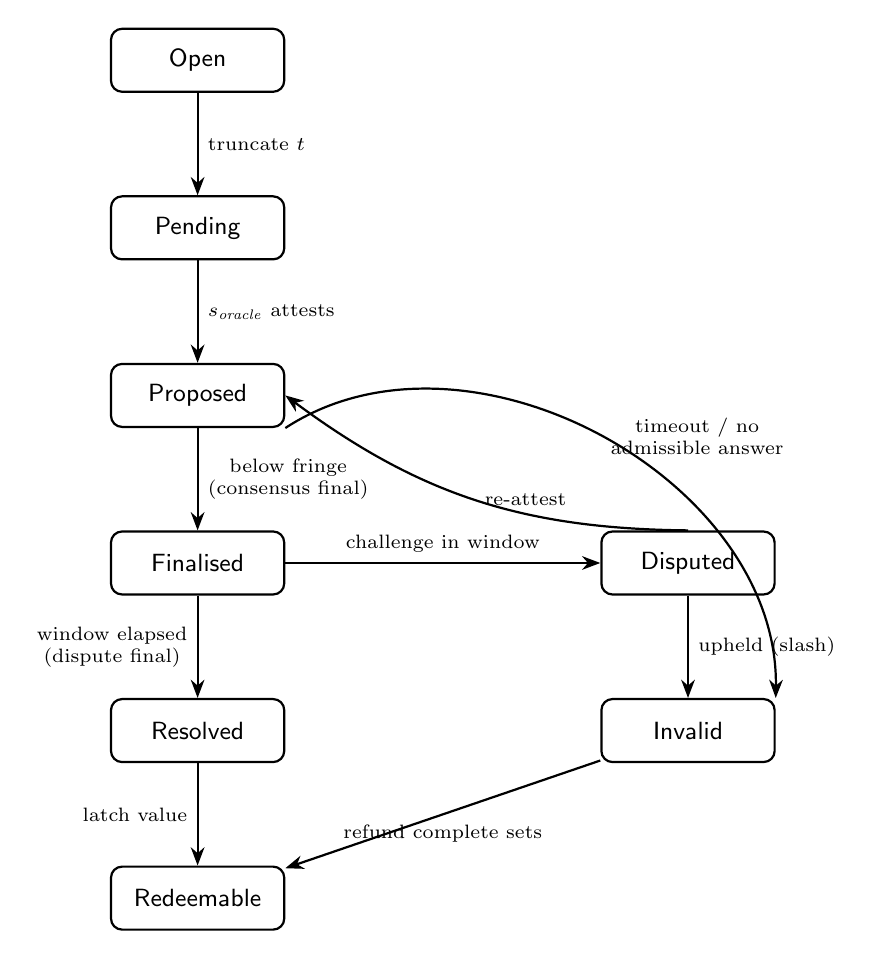
\begin{tikzpicture}[
  node distance=13mm and 40mm,
  state/.style={rectangle,rounded corners,draw,thick,minimum height=8mm,minimum width=22mm,font=\small\sffamily,align=center},
  every edge/.style={draw,thick,->,>=Stealth},
  lbl/.style={font=\scriptsize,align=center}
]
% main spine, vertical, left column
\node[state] (open) {Open};
\node[state,below=of open] (pending) {Pending};
\node[state,below=of pending] (proposed) {Proposed};
\node[state,below=of proposed] (finalised) {Finalised};
\node[state,below=of finalised] (resolved) {Resolved};
\node[state,below=of resolved] (redeem) {Redeemable};
% side branches, right column
\node[state,right=of finalised] (disputed) {Disputed};
\node[state,right=of resolved] (invalid) {Invalid};

% spine transitions
\draw (open) edge node[lbl,right]{truncate $t$} (pending);
\draw (pending) edge node[lbl,right]{$s_{\mathit{oracle}}$ attests} (proposed);
\draw (proposed) edge node[lbl,right]{below fringe\\(consensus final)} (finalised);
\draw (finalised) edge node[lbl,left]{window elapsed\\(dispute final)} (resolved);
\draw (resolved) edge node[lbl,left]{latch value} (redeem);

% branch transitions
\draw (finalised) edge node[lbl,above]{challenge in window} (disputed);
\draw (disputed) edge node[lbl,right]{upheld (slash)} (invalid);
\draw (disputed.north) edge[bend left=18] node[lbl,right]{re-attest} (proposed.east);
\draw (invalid) edge node[lbl,below]{refund complete sets} (redeem);
\draw (proposed.south east) edge[bend left=62] node[lbl,right]{timeout / no\\admissible answer} (invalid.north east);
\end{tikzpicture}
\caption{The resolution-latch state machine. Redeem is reachable only through \textsc{Resolved}
(a winning-share payout) or \textsc{Invalid} (a complete-set refund), and \textsc{Resolved} is
reachable only after both consensus finality (\textsc{Proposed}$\to$\textsc{Finalised}) and
dispute finality (\textsc{Finalised}$\to$\textsc{Resolved}).}
\label{fig:latch}
\end{figure}

\paragraph{Guards, precisely.}
\begin{itemize}[leftmargin=1.4em,itemsep=0.15em]
\item \textsc{Open}$\to$\textsc{Pending}: block height $\ge$ \textit{schedule}.close
($\textsf{truncate}\ t$). New trades refused; existing positions intact.
\item \textsc{Pending}$\to$\textsc{Proposed}: a message on the resolution channel $x$ signed
by \textit{authority} ($s_{\mathit{oracle}}$, or $s_{\mathit{oracle}}\sep s_{\mathit{compliance}}$),
carried in a validator-signed block. The attestation must be \emph{admissible} against
\textit{spec} (in the answer set; for a categorical market, exactly one slot).
\item \textsc{Proposed}$\to$\textsc{Finalised}: the proposing block is below the finality
fringe. The dispute clock starts \emph{here}, in finalised time.
\item \textsc{Proposed}$\to$\textsc{Invalid}: no admissible attestation arrived before
\textit{schedule}.horizon (timeout), or the attestation names no admissible outcome.
\item \textsc{Finalised}$\to$\textsc{Disputed}: a bonded challenge within the window. For a
distributional oracle this includes aggregate-distribution evidence
(Section~\ref{sec:oracle-spec}); the challenge bond funds the reconciliation and is forfeit if
the challenge fails.
\item \textsc{Disputed}$\to$\textsc{Proposed} or $\to$\textsc{Invalid}: reconciliation either
re-attests a corrected value (and the dispute clock restarts in finalised time) or upholds
invalidity (and the offending validator is slashed, Casper-style).
\item \textsc{Finalised}$\to$\textsc{Resolved}: the dispute window elapsed with the value
standing. \emph{The value is latched here, write-once.}
\item \textsc{Resolved}$\to$\textsc{Redeemable} and \textsc{Invalid}$\to$\textsc{Redeemable}:
the redeem gate opens. By Invariant~\ref{inv:nest} this is downstream of both finalities.
\end{itemize}

\subsection{The latch in rho}

Listing~\ref{lst:latch} sketches the latch as a one-shot write-once cell whose redeem branch is
gated on the conjunction of the two finalities, with the invalid branch refunding complete sets.

\begin{lstlisting}[caption={The resolution latch: write-once, redeem nested below consensus
and dispute finality, invalid refunds complete sets.},label={lst:latch}]
// latch(x, spec, authority, disputeWin, schedule, marketPurses):
//   x          - resolution channel (the oracle)
//   spec       - admissibility predicate + stratum + window policy
//   authority  - resolver capability (s_oracle [* s_compliance])
//   marketPurses - located purses holding the locked collateral
contract latch(@x, @spec, @authority, @disputeWin, @schedule, @mp) = {
  new resolved, invalidCh in {
    // PENDING -> PROPOSED: accept only an admissible, authorised attestation
    for (@(value, sig, blk) <- x) {
      match (authorised(sig, authority) and admissible(value, spec)) {
        false => invalidCh!("inadmissible or unauthorised")
        true  => {
          // PROPOSED -> FINALISED: wait until blk is below the fringe.
          // finalityFringe is the same boundary the GC maintains.
          for (_ <- finalityFringe!?(blk)) {
            new clock in {
              // dispute window measured in FINALISED time from here
              startFinalisedClock!(disputeWin, *clock) |
              select {
                // a challenge within the window -> reconciliation
                for (@chal <- disputeCh(blk)) {
                  reconcile!(chal, x, *invalidCh)   // may re-attest or slash
                }
                // window elapsed, value stands -> RESOLVED (latch, once)
                for (_ <- clock) {
                  resolved!(value)                  // write-once cell
                }
              }
            }
          }
        }
      }
    } |
    // REDEEMABLE via RESOLVED: winning shares -> collateral
    for (@v <- resolved) {
      openRedeem!(mp, v)        // pay holders of the winning outcome
    } |
    // REDEEMABLE via INVALID: complete sets -> collateral, first-class path
    for (@reason <- invalidCh) {
      openRefund!(mp, reason)   // every complete set redeems at par
    }
  }
}
\end{lstlisting}

\noindent The \texttt{resolved} channel is consumed once; a second attestation finds it empty
and cannot overwrite the latched value (the one-shot invariant of Section~\ref{sec:floor}). The
redeem gate's \texttt{finalityFringe} test is read-only access to the consensus liveness
boundary; the dispute clock's \texttt{startFinalisedClock} keys the window to finalised time,
discharging Invariant~\ref{inv:nest} structurally.

\section{Implementation roadmap}\label{sec:impl}

We collect the build into a primitive-by-primitive mapping (Table~\ref{tab:map}), a conservation
invariant the position layer must maintain, and a phased plan. The organising claim is that no
field of the configuration tuple requires a primitive outside cost-accounted rho plus the
combinators; the one new build, the maker, is engineering on the substrate.

\begin{table}[h]
\centering\small
\begin{tabular}{@{}p{3.5cm}p{5.3cm}p{4.4cm}@{}}
\toprule
\textbf{Venue component} & \textbf{F1R3Fi apparatus} & \textbf{Status} \\
\midrule
Outcome share & $\textsf{scale}(o,\textsf{one}(k))$, $o$ a latched observable & exists \\
\textsf{split} / \textsf{merge} & acceptance-gate reservations over located purses; conservation $=$ funding proof & exists (as gate); thin wrapper new \\
\textsf{redeem} & gated transfer, guarded by the latch & wrapper new \\
$N$-way / scalar partition & spatial-type fact; $\sum$ over slots & new (small) \\
Resolution observable & persistent oracle channel (\S\ref{sec:oracle-channel}) & exists \\
Resolution latch & one-shot write-once cell (\S\ref{sec:latch}) & new \\
Oracle provenance & $s_{\mathit{oracle}}$ as name; signatures-as-names & exists \\
Blame capability & $s_{\mathit{validator}}$ on the block; Casper accountable safety & exists (consensus) \\
Dispute window & finality-fringe read; same boundary as GC & exists (read-only); policy new \\
Maker (CPMM/LMSR) & inventory on located purses; gate per quote & new (the build) \\
Order book & resting funded comprehensions on a book channel & new \\
Order cancellation & object-capability receive on the order purse & exists (idiom) \\
Batch clearing & join over disjoint pools; uniform price & new \\
Compliance gate & $\{\mathsf{transfer}\}_{s_{\mathit{party}}\sep s_{\mathit{compliance}}}$ & exists \\
Audit trail & native ledger of funded rendezvous & exists \\
Position limits & $\Phi_{\mathrm{sep}}$, spatial bounds \cite[\S8]{finrho} & type layer (in progress) \\
Schedule (open/close/horizon) & \textsf{truncate} / \textsf{get} & exists \\
\bottomrule
\end{tabular}
\caption{Primitive-by-primitive map. ``exists'' means present in the realisation
of~\cite{finrho} or the consensus layer; ``new'' means to be built, with the build's nature
noted.}
\label{tab:map}
\end{table}

\begin{invariant}[Position-layer conservation]\label{inv:cons}
At every reachable state of a market, the collateral locked in the market's collateral purse
equals the number of outstanding complete sets, where a complete set is one share of each
outcome slot:
\[
\mathit{collateral} \;=\; \sum_{\text{minted}} 1 \;-\; \sum_{\text{merged}} 1 \;-\; \sum_{\text{redeemed}} 1,
\qquad
\bigl(\textstyle\bigsep_i \mathsf{purse}_i\bigr) \models \Phi_{\mathrm{sep}}.
\]
\textsf{split} increments outstanding sets and locks one unit of collateral; \textsf{merge}
decrements and releases one; \textsf{redeem} (post-latch) decrements and releases to the
holder of the winning slot (or, in the invalid case, to the holder of any complete set). Each
is one acceptance-gate reservation, so the invariant is the gate's linear funding proof and is
maintained by construction. $\Phi_{\mathrm{sep}}$---the purses do not alias---is the static
no-double-spend.
\end{invariant}

\subsection{A phased plan}

\paragraph{Phase 0 --- position layer.} Implement \textsf{split}/\textsf{merge}/\textsf{redeem}
over located purses for the binary partition, with Invariant~\ref{inv:cons} as the test oracle.
This is the smallest end-to-end slice and exercises the gate, the purses, and the conservation
law without any maker or live resolution. Resolve manually (a trusted key) to defer the oracle.

\paragraph{Phase 1 --- latch and oracle channel.} Implement the latch state machine
(Section~\ref{sec:latch}) with a deterministic oracle (a price feed or block height) and a
near-zero dispute window, exercising the consensus-finality read against the GC fringe. Add the
invalid/timeout branch and the complete-set refund. This makes resolution real on the easy
stratum before introducing dispute economics.

\paragraph{Phase 2 --- maker, batch-cleared.} Implement the order as a funded comprehension
(Listing~\ref{lst:order}) and the batch-clearing join (Listing~\ref{lst:batch}) with a CPMM or
LMSR residual. Start batch-cleared because it is the idiomatic, MEV-flat cell; add a continuous
mode later only if a specific market demands it, with the externality made explicit. Cancellation
is free (the object-capability idiom).

\paragraph{Phase 3 --- categorical and scalar partitions.} Generalise the position layer and the
maker to $N$-way and scalar markets. The conservation invariant generalises directly; the maker's
$\sum_j e^{q_j/b}$ (LMSR) or product (CPMM) ranges over the slots.

\paragraph{Phase 4 --- dispute economics and distributional oracles.} Add the bonded-challenge
game, the reconciliation/slashing path, and distributional-oracle specifications with
aggregate-distribution challenges. This is where the genuinely non-deterministic oracles (the
high-temperature language model) become usable, and where the design risk is concentrated; it is
deliberately last, after the easy strata work end-to-end.

\paragraph{Phase 5 --- compliance and limits.} Add the $\mathsf{Gated}(s_{\mathit{compliance}})$
configuration and position limits, lifting the regulated-venue bundle. The compliance gate and
audit trail already exist; this phase wires them into the market template and the launch tuple.

\paragraph{Configuration surface.} Throughout, the market template is parameterised by the
tuple of Section~\ref{sec:tuple}, with the dependent edges enforced as coherent bundles and the
floor of Section~\ref{sec:floor} fixed. A launch is the instantiation of the template at a
type-checked record.

\section{Conclusion}\label{sec:conclusion}

A financial contract is a thing one holds; a prediction market is a place one trades. The
combinators, realised in the cost-accounted rho calculus, already give the first. We have shown
that the second is mostly within reach of the same apparatus: the position layer is located
purses and the acceptance gate, with conservation as the funding proof; the oracle is a trusted
computation behind a channel, with non-repeatable calls secured by validator attribution---a
blame capability Casper already supplies---rather than by a replicated determinism that genuinely
non-deterministic oracles cannot provide, and with the oracle's declared specification furnishing
the falsification surface that lets blame attach; the market launch is a single dependent
configuration tuple over a fixed safety floor; the maker is two orthogonal axes whose
batch-cleared cell is idiomatic to the substrate's concurrency discipline; and the
resolution latch nests redeem below both consensus finality (the same fringe the runtime
garbage-collects against) and dispute finality (a window in finalised time). The one genuinely
new build is the maker, and it is engineering on the substrate rather than an extension of it.
A description language tells you what a contract is worth; a settlement language on this
substrate tells you, before a token moves, that it will settle; and a venue on this substrate
tells you, before a market opens, the exact discipline under which it will trade and resolve.

\subsection*{Acknowledgements}
This note develops work conducted in extended dialogue with Anthropic's Claude, which served as
a sounding board throughout---separating the venue layers, pressing on the oracle-determinism
question until attribution rather than replication emerged as the right invariant, and drawing
out the configuration tuple and the latch nesting. The ideas and any errors are the author's.

\begin{thebibliography}{9}
\small
\bibitem{spj} S.\ Peyton Jones, J.-M.\ Eber, J.\ Seward. Composing contracts: an adventure in
financial engineering (functional pearl). ICFP, Montreal, 2000.
\bibitem{finrho} L.\ G.\ Meredith. Financial Contract Combinators in the Cost-Accounted Rho
Calculus. F1R3FLY.io, 2026.
\bibitem{cost} L.\ G.\ Meredith. Cost-accounted rho calculus: a spectral decomposition of
phlogiston. F1R3FLY.io, 2026.
\bibitem{cigslt} L.\ G.\ Meredith. Continued interactive GSLTs and the cost endofunctor: a
construction one level up from cost-accounted Rholang. F1R3FLY.io, 2026.
\bibitem{rholang} L.\ G.\ Meredith et al. Rholang specification. F1R3FLY.io / RChain
Cooperative, 2017--2026.
\bibitem{casper} V.\ Buterin, V.\ Griffith. Casper the Friendly Finality Gadget.
arXiv:1710.09437, 2017.
\bibitem{hanson} R.\ Hanson. Logarithmic market scoring rules for modular combinatorial
information aggregation. Journal of Prediction Markets 1(1):3--15, 2007.
\bibitem{ctf} Gnosis. Conditional Tokens Framework. \texttt{docs.gnosis.io}, 2019.
\bibitem{uma} UMA. Optimistic Oracle. \texttt{docs.uma.xyz}, 2021.
\bibitem{mev} P.\ Daian et al. Flash Boys 2.0: frontrunning, transaction reordering, and
consensus instability in decentralized exchanges. IEEE S\&P, 2020.
\end{thebibliography}

\end{document}
